%% Draft v0.2, 7 Oct 2026. Results sections hold placeholders marked \todo{}.
\documentclass[11pt,letterpaper]{article}
\usepackage[margin=1in]{geometry}
\usepackage[T1]{fontenc}
\usepackage[utf8]{inputenc}
\usepackage{newtxtext,newtxmath}
\usepackage{microtype}
\usepackage{graphicx}
\usepackage{booktabs}
\usepackage{float}
\usepackage{array}
\usepackage{xcolor}
\usepackage{amsmath}
\usepackage[numbers,sort&compress]{natbib}
\usepackage[hidelinks,pdftitle={Teaching Robots to Handle Knives Safely Around People},pdfauthor={Abdulahad Nabiev}]{hyperref}
\usepackage{caption}
\captionsetup{font=small,labelfont=bf,width=0.95\textwidth}
\usepackage{setspace}
\setstretch{1.04}
\usepackage{authblk}
\renewcommand\Authfont{\normalsize}
\renewcommand\Affilfont{\small\itshape}
\usepackage{titlesec}
\titlespacing*{\paragraph}{0pt}{0.9ex plus 0.3ex minus 0.2ex}{1em}
\usepackage{enumitem}
\setlist{nosep}
\usepackage[section]{placeins}

\newcommand{\pct}{\,\%}
\newcommand{\todo}[1]{{\color{red}[#1]}}

\title{\Large\bfseries Teaching Robots to Handle Knives Safely Around People:\\ A Simulation Benchmark for Sharp-Tool Manipulation}
\author[1]{Abdulahad Nabiev}
\affil[1]{Independent researcher, Tashkent, Uzbekistan\\ \texttt{n.abdulahadferps@gmail.com}}
\date{Draft, October 2026}

\begin{document}
\maketitle
\thispagestyle{empty}

\begin{abstract}
\noindent
Robots that help in homes, hospitals and care facilities will have to use kitchen tools next to people. A knife in a robot's hand is a new kind of hazard: the robot can keep its whole body away from a person and still point a blade at their arm. Today's safety rules and training benchmarks for robots that work near people only check whether the robot's body touches the person, so they cannot see this. This paper gives robots a way to be measured, and trained, on how they handle a sharp tool near a person. We define four simple numbers that can be computed in any simulator: how far the blade's edge is from the nearest part of the person, whether the sharp side is facing them, how fast the edge is moving toward them, and a combined hazard score that adds up over time. We then build five kitchen tasks in simulation with a six-joint robot arm, a rigid knife and a person reaching into the workspace: carrying the knife, putting it down while a hand approaches, chopping while a hand enters the board, handing the knife over handle first, and passing the knife by a resting arm. \todo{We train reinforcement-learning policies with the usual body-contact penalty and show that they succeed X\pct{} of the time with Y\pct{} body contacts, yet in Z\pct{} of their successful runs the edge faces the person within 5~cm. Adding our hazard score to the training signal cuts that exposure by A\pct{} at a cost of B points of success.} The tasks, the metrics and the knife model are released as a small module that plugs into existing MuJoCo environments, so that other groups can measure the same thing on their own robots.
\end{abstract}

\vspace{1em}
\noindent\textbf{Keywords:} assistive robots, human-robot collaboration, sharp tools, safety, reinforcement learning, simulation benchmark

\vfill
\noindent\small Code, tasks and evaluation logs: \url{https://github.com/abdulahad2008/piper_simulation}
\normalsize
\newpage
\setcounter{page}{1}

\begin{figure}[t]
\centering
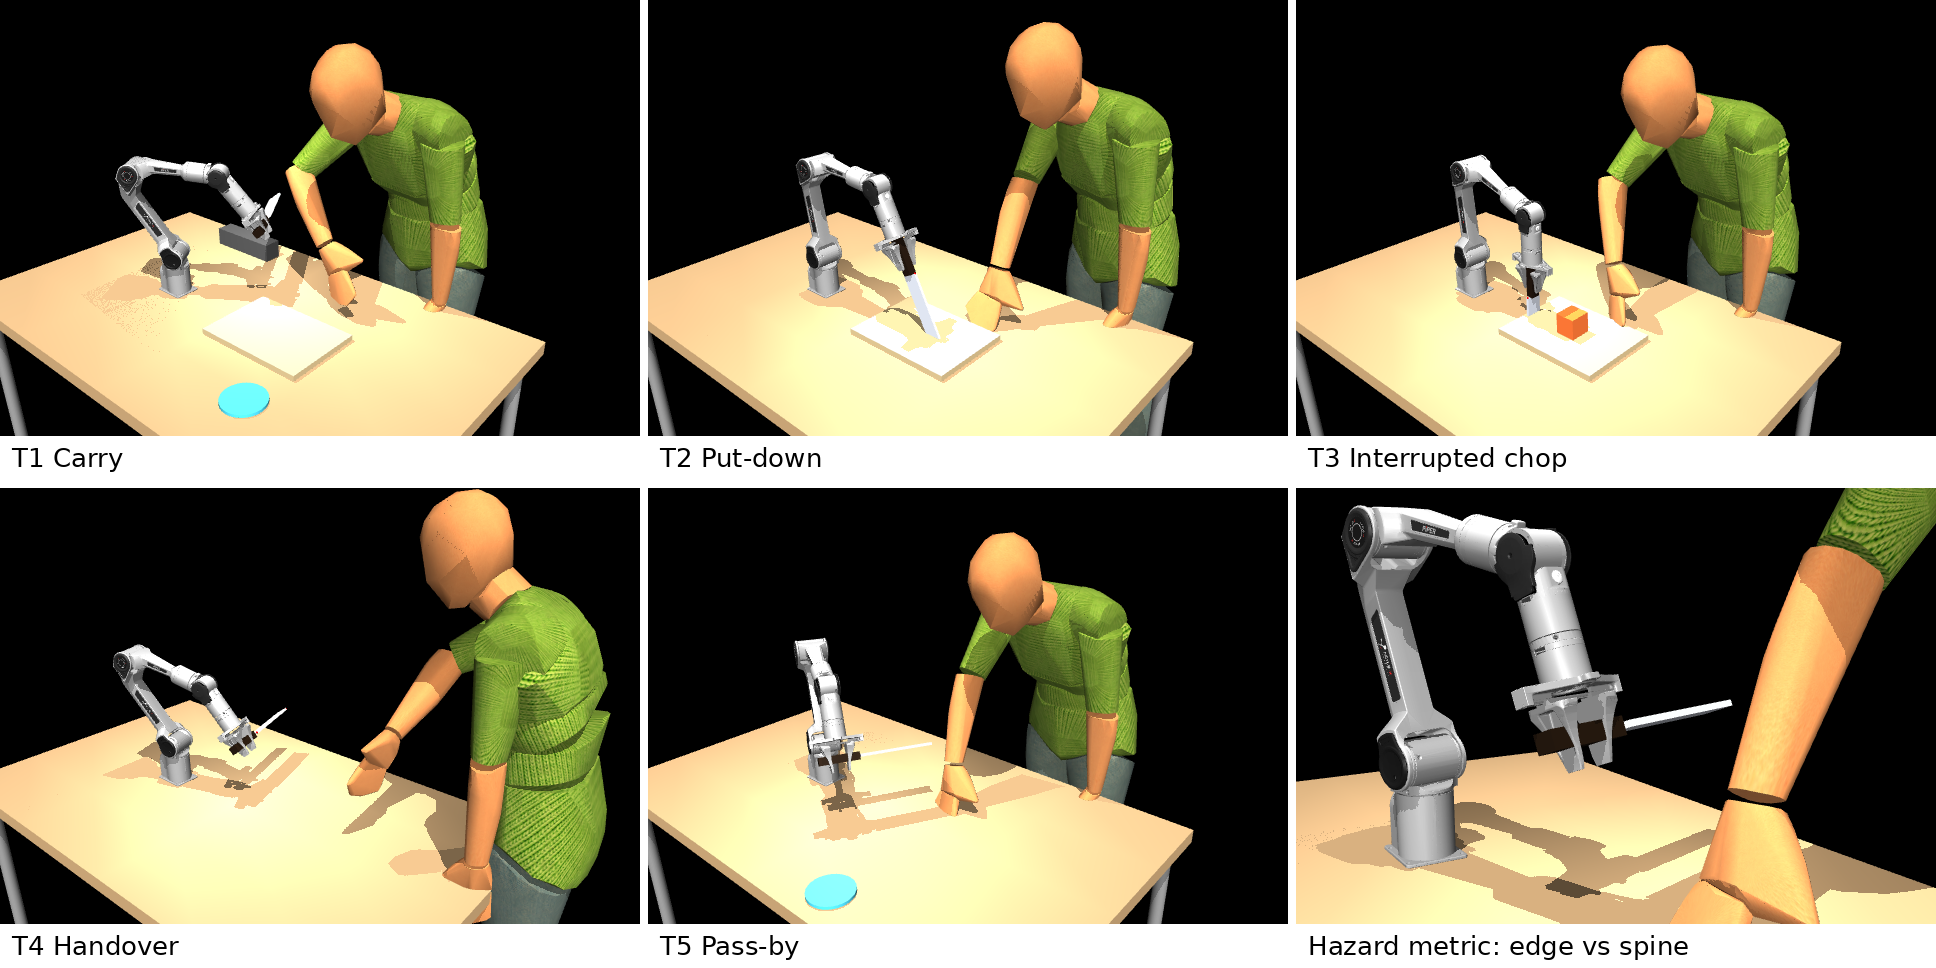
\includegraphics[width=\textwidth]{fig_tasks.png}
\caption{The five tasks and the hazard metric, rendered from the simulator. A six-joint arm holds a rigid chef's knife on a table while a simulated person reaches into the workspace. T1 carry the knife across the table; T2 put the knife down as a hand approaches; T3 chop a block while a hand enters the board; T4 hand the knife over handle first; T5 pass the knife by a resting or moving arm. Bottom right: the quantity the paper measures, the distance and orientation of the blade's edge relative to the person's forearm. The human model is the one used in Human-Robot Gym \cite{thumm2024humanrobotgym}; poses are illustrative.}
\label{fig:tasks}
\end{figure}

\section{Introduction}
The robots now being built to assist people, humanoids and arms in homes and care settings, will have to handle the same objects people do, and many of those objects are sharp. Cutting food, clearing a table, passing a pair of scissors or a knife: these are ordinary tasks for a person and dangerous ones for a robot that does not understand what it is holding.

Safety for robots working near people is currently defined around the robot's body. The collaborative-robot standards limit the speed, the separation and the energy with which a robot link may contact a person \cite{iso10218,iso15066,haddadin2009requirements}, and the learning benchmarks that train robots next to people keep the same definition. Human-Robot Gym \cite{thumm2024humanrobotgym} trains policies beside motion-captured humans under a shield that keeps every robot link inside those limits \cite{thumm2022provably}. HRIBench \cite{liu2026hribench} scores collision-free rate and contact safety between the robot and a human avatar. In both, whatever the gripper holds is either absent or treated as a blunt extension of the last link.

In a kitchen the object in the gripper is often the hazard. A robot carrying a chef's knife can keep every link ten centimetres from a person and still hold the edge against their forearm. The same motion with the spine of the blade toward the person is harmless. A body-contact metric reports the two cases as identical, and a shield that reasons about links permits both. Tool-aware collision avoidance adjusts the robot's swept volume for the size of the tool \cite{toolaware2025collision}, which keeps the tool from touching anything, but it does not distinguish the edge from the spine, or the approach speed of the edge from its lateral speed.

This paper makes the hazard of a held sharp tool measurable and gives learning methods something to be measured on. The contribution has three parts.

\begin{enumerate}[leftmargin=1.5em]
\item \textbf{Metrics.} For a rigid tool with a known edge we define the edge distance $d$, the edge alignment $a$, the closing speed $v$, and an instantaneous hazard $h$ that is zero when the edge is far or pointed away and grows with proximity, alignment and approach speed. Integrated over an episode, $h$ gives an exposure time $E$ in seconds. The definitions need only the tool pose and a capsule model of the person, so they apply unchanged to motion-capture data and to any simulator.
\item \textbf{Tasks.} Five kitchen tasks on a six-joint arm with a rigid knife and a simulated person (Figure~\ref{fig:tasks}): carry, put-down, interrupted chopping, handover and pass-by, each with pre-registered held-out human-motion suites.
\item \textbf{Baselines.} \todo{Reinforcement learning with the conventional body-contact reward, the same with a hazard-shaped reward, a constrained learner with a budget on exposure, and a body-only safety shield. The first and last show the problem; the middle two show how much of it the metric removes.}
\end{enumerate}

We make no claim about cutting physics. The knife is rigid and chopping is a kinematic event. The question is whether a learned policy keeps the edge away from the person, and that question is about the pose and the velocity of a rigid body. The long-term aim is plain: assistive and humanoid robots will be trusted with sharp tools only when their training and their evaluation can see the tool.

\section{Related work}
\paragraph{Safety in physical human-robot interaction.}
Speed and separation monitoring and power and force limiting are the two operating modes of the collaborative-robot standards \cite{iso10218,iso15066}, and both are stated for the robot's links with the tool as a rigid extension of the flange. The biomechanical studies behind them measure injury from blunt impact and clamping \cite{haddadin2009requirements}. Lasota et al.\ survey the field \cite{lasota2017survey}. Shields filter a learned policy's actions so that no unsafe command is executed \cite{alshiekh2018shielding,thumm2022provably}, and safe reinforcement learning constrains the learning problem itself \cite{garcia2015safe}. None of this work models the edge of a held tool as distinct from its volume.

\paragraph{Benchmarks with humans in the scene.}
Human-Robot Gym \cite{thumm2024humanrobotgym} provides eight tasks with motion-captured humans and a provable shield, and reports success, reward and collision. HRIBench \cite{liu2026hribench} generates human avatars with a motion model and scores collision-free rate, human contact safety and recovery after a disruption; its intruder tasks, in which a person interrupts the robot, are where current policies fail. Collaborative hammering in Human-Robot Gym is the one task in either benchmark with a tool, and the tool is treated as a blunt object. Our tasks are closest to HRIBench's intruder setting with a sharp tool, and to Human-Robot Gym's handover tasks with the orientation of the object made to matter.

\paragraph{Safe reinforcement learning benchmarks.}
Safety Gym \cite{ray2019safetygym} and Safety-Gymnasium \cite{ji2023safetygymnasium} established the cost signal and the constrained-policy baselines \cite{achiam2017cpo,ji2024omnisafe} that we use. Safety-Gymnasium's dexterous-hand tasks and ReDMan \cite{geng2025redman} constrain the hand and the object, with no person in the scene. Our hazard $h$ is a cost signal in exactly their sense and plugs into their algorithms.

\paragraph{Robotic cutting.}
DiSECt \cite{heiden2021disect} and SliceIt! \cite{beltran2024sliceit} simulate the interaction between a blade and food for learning cutting skills. They model the material, not the bystander. We use a rigid knife and a kinematic slice event so that the cost of simulation stays at the level of a rigid-body benchmark.

\paragraph{Handover and perceived danger.}
Reviews of object handover \cite{ortenzi2021handovers} and the finding that receivers prefer a visible handle \cite{ortenzi2022handle} motivate our handover task. A database of kitchen objects rated for perceived danger \cite{leusmann2023database} and a study of how perceived danger changes handover distance \cite{perceiveddanger2025handover} measure the human side of the problem with user studies. We take the orientation rule they support, handle toward the receiver and edge away, and turn it into a measurable success condition for a learned policy.

\paragraph{Tool-aware control.}
Tool-aware collision avoidance \cite{toolaware2025collision} filters the tool out of a point cloud and expands the robot's avoidance volume to match it. It handles the size of the tool and not its edge. The freezing-robot problem \cite{trautman2010unfreezing} is relevant to our interrupted-chopping task: a policy that stops with the edge in a person's path is safe by a body metric and not by ours.

\paragraph{Shortcut learning in robot policies.}
Policies trained on narrow data can succeed for the wrong reason \cite{geirhos2020shortcut,xing2025shortcut,wen2020copycat}. Our held-out human-motion suites and the no-human control are designed with that in mind: a policy that only ever saw one person's motion may keep the edge clear by timing rather than by understanding, and the suites are there to tell the two apart.

\section{Hazard model}
\label{sec:hazard}
\paragraph{Tool.}
A rigid sharp tool is described by its edge, a segment from heel $\mathbf{p}_h$ to tip $\mathbf{p}_t$ in the world frame, and by a unit cutting direction $\mathbf{c}$ that points out of the sharp side, perpendicular to the edge and in the plane of the blade. For a chef's knife the edge is the lower boundary of the blade and $\mathbf{c}$ points down when the knife rests on a board. Both are fixed in the tool frame and move with it. Tools with more than one edge are described by a list of edges and the maximum is taken.

\paragraph{Person.}
The person is a set of capsules, each a segment with a radius. This is how the simulated forearm and hand are built in our environment and how the body parts are represented in Human-Robot Gym. Any skeleton with limb radii can be converted.

\paragraph{Per-step quantities.}
Let $\mathbf{q}_e$ and $\mathbf{q}_p$ be the closest points between the edge segment and the surface of the nearest capsule, and $\mathbf{u}$ the unit vector from $\mathbf{q}_e$ to $\mathbf{q}_p$.
\begin{align}
d &= \lVert \mathbf{q}_p - \mathbf{q}_e \rVert - r \quad\text{(signed; } d \le 0 \text{ is a cut)}\\
a &= \max(0,\, \mathbf{c}\cdot\mathbf{u})\\
v &= \max\bigl(0,\, (\dot{\mathbf{q}}_e - \dot{\mathbf{q}}_p)\cdot\mathbf{u}\bigr) \;\text{ if } a > 0,\; 0 \text{ otherwise}\\
h &= a\,\Bigl(1 + \frac{v}{v_0}\Bigr)\,\max\Bigl(0,\, 1 - \frac{d}{d_0}\Bigr)
\end{align}
where $r$ is the capsule radius, $d_0$ is the distance beyond which the edge is considered harmless and $v_0$ scales the approach speed. We fix $d_0 = 0.15$~m and $v_0 = 0.25$~m/s before any experiment and report sensitivity to both in the appendix. $h$ is zero whenever the edge is farther than $d_0$, or the spine or the flat faces the person. It is at least $1$ when the edge touches the person squarely and larger when it is also approaching.

\paragraph{Episode quantities.}
The exposure $E = \sum_t h_t\,\Delta t$ is the hazard-weighted time, in seconds, that the person spent near a facing edge. We also report the minimum edge distance, the maximum hazard, the maximum closing speed, the fraction of steps with $a > 0.5$ and $d < d_0$, and a cut flag ($d \le 0$ at any step). Margins are reported conditioned on success, because an episode that ends in a cut is never counted among the successes.

\paragraph{What the model leaves out.}
$h$ does not model the force needed to cut skin, the sharpness of the blade or the compliance of the arm. It is a geometric and kinematic proxy. The argument for it is the same as for separation distance in the standards: it is measurable in every simulator and on every motion-capture rig, it is zero in every situation a person would call safe, and it is large in every situation a person would call dangerous. Figure~\ref{fig:demo} shows the two cases the model separates and a body-contact metric does not.

\begin{figure}[t]
\centering
\todo{Figure: the same knife sweep past a forearm, edge toward and spine toward the person; traces of $d$, $a$, $v$ and $h$ below each. Generated by \texttt{scripts/demo\_hazard.py}.}
\caption{Two passes along the same path at the same speed with no contact. A body-contact metric reports nothing in either. With the edge toward the forearm the exposure is $1.15$~s and the peak hazard $1.06$; with the spine toward the forearm both are zero.}
\label{fig:demo}
\end{figure}

\section{Tasks}
\label{sec:tasks}
\paragraph{Scene.}
A six-joint AgileX PiPER arm \cite{agilexpiper,zakka2022menagerie} in MuJoCo \cite{todorov2012mujoco} at 20~Hz control over 500~Hz physics, with a five-dimensional Cartesian action (tool displacement, wrist yaw rate, gripper command). The knife is a rigid body with a 200~mm blade and a 110~mm handle, welded to the tool frame once grasped. The simulated person is a forearm and hand built from capsules that move on minimum-jerk trajectories between waypoints, drawn from a distribution over five trajectory types (crossing the workspace, reaching toward the object, reaching toward the target, crossing with a pause, entering and reversing), appearance time, speed, side, hand height and closest approach to the task centreline. The policy observes the robot's proprioception and task state, a human block (presence flag, hand position and velocity, elbow position, tool-to-hand vector), and nine blade channels: the heel, the tip and the cutting direction in the base frame. An episode ends on success, on a body contact, on a cut, or after 200 steps.

\paragraph{The five tasks.}
\begin{description}[leftmargin=1.5em]
\item[T1 Carry.] Pick the knife from a rack pose, carry it across the board and place it on a target pad with the edge down, while the person reaches across the workspace.
\item[T2 Put-down.] The knife starts in the gripper. A hand reaches toward the board at a random time. Place the knife on the board with the edge away from the person's side and retract the gripper at least 0.2~m.
\item[T3 Interrupted chop.] Chop a block with repeated strokes. A slice is counted when the edge passes through the block's cutting plane. A hand enters the board region and reverses, with pauses. Success is a fixed number of slices with no cut and no body contact.
\item[T4 Handover.] Present the knife to the person's hand handle first and release when the hand closes on the handle. Success requires the handle inside the hand capsule and $a \le 0$ with respect to the hand at release.
\item[T5 Pass-by.] Carry the knife from one side of the table to the other while the person's arm rests across the path or moves across it.
\end{description}
T1 and T5 are plain pick-and-place with a tool, and exist to show that the body metric and the edge metric disagree on policies that are good by the body metric. T2 and T4 make the orientation of the knife part of success. T3 is the intruder setting of HRIBench with a blade, and is where stopping and retracting differ.

\paragraph{Held-out suites.}
Each task has six held-out suites fixed in a manifest before any multi-seed run: no person present (a check that $E$ is zero when nobody is there), the training crossing exactly, the training crossing shifted in time, speed and distance, randomised in-distribution motion with seeds disjoint from training, out-of-distribution motion from the other side with 150~ms observation latency, and a counterfactual pair in which the person is shown to the policy but absent from the scene, or present in the scene but hidden from the policy. The last pair separates a policy that avoids the person from one that uses the sight of the person as a timing cue.

\section{Learners}
\label{sec:learners}
All policies are soft actor-critic \cite{haarnoja2018sac} in Stable-Baselines3 \cite{raffin2021sb3}, 256$\times$256 networks, 2~M environment steps, three seeds per regime, with checkpoint selection on a validation seed that is disjoint from every test seed. Four regimes are trained.
\begin{description}[leftmargin=1.5em]
\item[R0 Body reward.] The conventional reward: task shaping, a proximity penalty on the tool centre point and a body-contact penalty of 100. The knife is in the scene and in the observation but not in the reward.
\item[R1 Hazard-shaped.] R0 minus $2\,h_t$ per step.
\item[R2 Constrained.] R0 as the reward and $h_t$ as the cost, trained with SAC-Lagrangian \cite{ji2024omnisafe} under the constraint $E \le 0.1$~s per episode.
\item[R3 Body shield.] The R0 policy executed under a stop shield that halts the arm when any link's predicted separation from the person falls below a threshold, in the manner of speed and separation monitoring, with no knowledge of the knife.
\end{description}
R0 and R3 are the two ways the field currently handles the problem. R1 and R2 are the minimum change that uses the metric.

\section{Evaluation protocol}
Primary outcomes, fixed before the multi-seed runs: task success $S$, body-contact rate $C$, cut rate $K$, exposure $E$, and the 5th percentile of the minimum edge distance over successful episodes, all on the randomised in-distribution and out-of-distribution suites. Two pre-registered hypotheses:
\begin{description}[leftmargin=1.5em]
\item[H1.] R0 policies reach high success and low body-contact rate on T1 and T5, and their cut rate and exposure are not lower than those of a control that holds the knife at a random fixed orientation.
\item[H2.] R1 and R2 reduce exposure by at least half relative to R0 at a cost of fewer than ten points of success on the randomised suite.
\end{description}
Rates carry Wilson intervals over episodes within a seed; regimes are summarised as the range over seeds; paired counterfactual differences carry bootstrap intervals over episode pairs. Every number is recomputed from committed per-episode logs.

\section{Results}
\todo{To be filled after the runs. Planned tables: (1) $S$, $C$, $K$, $E$ per regime and task on the two primary suites; (2) margin table conditioned on success, body separation beside edge distance; (3) counterfactual table for R0 and R2; (4) sensitivity of the ranking of regimes to $d_0$ and $v_0$.}

\subsection{Body-safe and edge-unsafe}
\todo{The headline result for T1/T5: R0 and R3 have low $C$ and high $S$, and nonzero $K$ and $E$. Report what fraction of successful R0 episodes had the edge facing the person within 5~cm, and the typical orientation the policy chose.}

\subsection{What the hazard cost buys}
\todo{R1 vs R2 vs R0: exposure reduction and success cost. Whether the constraint holds on held-out motion. Whether the policy learned to orient the knife (alignment falls) or to keep distance (edge distance rises).}

\subsection{Stopping with a knife}
\todo{T3: R3 freezes with the blade in the hand's path; R2 retracts. Hazard trace over the interruption for one episode of each.}

\subsection{Counterfactual suites}
\todo{Shown-but-absent and present-but-hidden person for R0 and R2: whether hazard-constrained policies also use the person as a timing cue.}

\section{Discussion and limitations}
\paragraph{Why a metric and not a controller.}
\todo{Rewrite after results.} A controller that keeps the knife away from people is the eventual goal. A metric comes first because without it no controller can be compared, and because the training signal that produces such a controller is the metric itself. The claim that a body-contact metric can be satisfied while an edge metric is violated holds by construction and is shown in Figure~\ref{fig:demo}; the experiments establish whether learned policies actually end up in that region, and how much a small change to the training signal moves them out of it.

\paragraph{Limitations.}
The knife is rigid and cutting is kinematic, so nothing here speaks to cutting force or blade sharpness. The person is a forearm and a hand, not a body. The arm is one six-joint platform with a parallel gripper; a humanoid hand changes the grasp but not the metric, which is defined on the tool pose. The hazard constants $d_0$ and $v_0$ are chosen, not measured, and we report sensitivity rather than a justification from injury data. Simulation only; the metric applies to real motion capture but we have not run it on a real robot.

\paragraph{Use of generative AI tools.}
\todo{Generative AI coding assistants were used to write and refactor code. All generated code was reviewed by the author. The study design, the pre-registered protocol, the training runs and the interpretation of the results are the author's own.}

\section*{Reproducibility}
The hazard module, the knife model, the task definitions and the pre-registered manifest are in the repository. Running the unit tests and \texttt{scripts/demo\_hazard.py} reproduces Figure~\ref{fig:demo} without training, and \texttt{scripts/render\_tasks.py} reproduces Figure~\ref{fig:tasks}.

\bibliographystyle{unsrtnat}
\bibliography{refs}

\appendix
\section{Sensitivity to $d_0$ and $v_0$}
\todo{Table: ranking of regimes by $E$ for $d_0 \in \{0.10, 0.15, 0.20\}$ and $v_0 \in \{0.15, 0.25, 0.40\}$.}

\section{Per-seed tables}
\todo{Per-seed values for every cell of the main tables.}

\end{document}
